\documentclass[a4paper]{article}
\usepackage[left=20mm, total={170mm, 257mm}, top=20mm]{geometry}
\usepackage[utf8]{inputenc}
\usepackage[czech]{babel}
%\usepackage{amsthm}
\usepackage{amsmath}
\usepackage{graphicx}
%\usepackage{enumitem}
%\usepackage[ruled, linesnumbered]{algorithm2e}
%\usepackage{tikz}
%\usetikzlibrary{automata, positioning, arrows}
\usepackage[hidelinks, colorlinks, linkcolor=blue]{hyperref}

\newcommand{\bigO}[1]{\mathcal{O}(#1)}

\makeatletter
\renewcommand\maketitle{
{\raggedright
\begin{center}
{\Large \bfseries \@title}\\[2ex]
{\@author}\\[8ex] 
\end{center}}}
\makeatother

\title{Paralelní a distribuované algoritmy (PRL) – 2022/2023\\[0.4ex] \large Projekt 2 -- Implementace paralelního algoritmu K-means}
\author{Domink Nejedlý (xnejed09)}

\begin{document}

\maketitle



\section{Rozbor a analýza algoritmu}



Implementovaný algoritmus 4-means řeší rozdělení vstupních hodnot do čtyř shluků podle toho, jak daleko od středu (počítán jako průměr hodnot, jež shluk obsahuje) daného shluku se nachází. V každé iteraci je každá hodnota zařazena do shluku, k jehož středu zaujímá nejkratší vzdálenost (absolutní hodnota rozdílu středu shluku a~dané hodnoty). Pokud pak mezi dvěma po sobě jdoucími iteracemi nedojde ke změně žádného středu ani jednoho ze všech čtyř shluků, je nalezeno řešení a výpočet končí. Jelikož implementovaný algoritmus pracuje se skalárními (jednorozměrnými) hodnotami a pouze čtyřmi shluky ($k = 4$) jistě konverguje v lineárním počtu provedených iterací (počet iterací je shora omezen lineárně) -- $\bigO{n}$ -- vzhledem k $n$ vstupním hodnotám. Tohle je dokázáno v článku \href{https://link.springer.com/chapter/10.1007/978-3-540-45167-9_56}{How Fast Is $k$-Means?} pro případ, kdy $k < 5$ a algoritmus pracuje se skalárními (jednorozměrnými) daty.

Rozeberme celkovou časovou a prostorovou složitost implementovaného algoritmu. Samotné načtení dat -- $n$ vstupních hodnot -- a vytištění výsledků hlavním procesem nemusíme uvažovat, jelikož obě tyto operace lze provést v lineárním čase $\bigO{n} + \bigO{4n} = \bigO{n}$. Pro vytištění výsledků je uvedeno $\bigO{4n}$ pro zdůraznění čtyř průchodů polem, které obsahuje identifikaci odpovídajícího shluku pro každé číslo (index tohoto pole odpovídá indexu odpovídající hodnoty v poli se vstupními hodnotami). Po načtení $n$ vstupních hodnot hlavním procesem dochází k inicializaci středů shluků (v konstantním čase, jelikož jsou vždy čtyři) -- $\bigO{1}$ -- a k distribuci načtených hodnot mezi všech $N$ běžících procesů. Je předpokládáno, že každý proces má na starosti právě jednu hodnotu, tedy $n = N$. K rozdělení hodnot mezi procesy je využita funkce \verb|MPI_Scatter|, jejíž časová složitost jistě nepřesáhne $\bigO{n}$. Následně dochází k běhu jednotlivých výpočetních iterací zajišťujících opakované rozřazování hodnot do shluků a přepočítávání středů těchto shluků. Nejprve jsou aktuální středy shluků (vždy pole o~čtyřech hodnotách) rozhlášeny z hlavního procesu mezi všechny ostatní procesy pomocí funkce \verb|MPI_Bcast| -- logaritmická časová složitost $\bigO{\log N}$. Následně je v konstantním čase ($\bigO{1}$) každým procesem odpovídající hodnotě určen patřičný shluk (pomocí indexu $0$-$3$ do pole se středy shluků) a následně jsou pomocí jedné redukce funkcí \verb|MPI_Reduce| získány do hlavního procesu ($0$) součty hodnot přiřazených do jednotlivých shluků. Ta je provedena v logaritmickém čase -- $\bigO{\log N}$. Další redukcí (funkcí \verb|MPI_Reduce|) jsou pak do hlavního procesu získány počty hodnot v jednotlivých shlucích -- opět s logaritmickou časovou složitostí $\bigO{\log N}$. Hlavní proces poté v~konstantním čase -- $\bigO{1}$ -- z těchto získaných hodnot vypočítá nové středy shluků a nastaví řídící proměnnou cyklu (v němž probíhají tyto iterace pro rozřazování prvků) \verb|doNextIter| podle toho, zdali se nějaký ze středů po přerozdělení hodnot změnil, či nikoli -- \verb|true|, pokud ke změně středu nějakého shluku došlo, jinak \verb|false|. Hodnota této řídící proměnné je pak v logaritmickém čase -- $\bigO{\log N}$ -- rozhlášena z hlavního procesu i~všem procesům ostatním (aby bylo zajištěno ukončení běhu tohoto cyklu i~v~nich). Po ukončení běhu tohoto cyklu je s využitím funkce \verb|MPI_Gather| v hlavním procesu shromážděna identifikace odpovídajícího shluku pro každou rozřazovanou vstupní hodnotu. Časová složitost tohoto kroku jistě nepřekročí $\bigO{n}$. Hlavní proces nakonec vytiskne všechny výsledky (v lineárním čase -- $\bigO{n}$ -- jak již bylo zmíněno) a výpočet je úspěšně ukončen.

Z popisu chování implementovaného algoritmu je zřejmé, že časová složitost, vzhledem k tomu, že $N = n$ (tedy počet procesů je roven počtu rozdělovaných hodnot), je
$$ \bigO{1} +  \bigO{n} +  \bigO{n}(\bigO{\log n} + \bigO{1} + \bigO{\log n} + \bigO{\log n} + \bigO{1} + \bigO{\log n}) + \bigO{n} = \bigO{n \log n} \text{ (linearitmická)},$$
jelikož časová složitost provedení jedné iterace je logaritmická ($\bigO{\log n}$) a jejich počet je omezen lineárně ($\bigO{n}$) -- časová složitost načtení vstupních hodnot a vytištění výsledků pak nemá na celkovou výslednou časovou složitost žádný vliv (ta bude i s nimi stále linearitmická -- $\bigO{n \log n}$).

Prostorová složitost algoritmu je pak lineární ($\bigO{n}$), jelikož počet procesorů $N = n$, kde $n$ je počet rozřazovaných hodnot a každý proces pracuje vždy pouze s jednou z nich, přičemž dále disponuje nějakou konstantní -- $\bigO{1}$ -- částí paměti pro uchování pomocných hodnot a středů shluků. Výjimkou je pak proces hlavní, který navíc obsahuje pole vstupních hodnot a na konci výpočtu pak ještě pole obsahující identifikaci odpovídajícího shluku pro každou vstupní hodnotu. Pokud je tedy prostorová složitost vyjádřena prostřednictvím těchto dílčích popsaných nároků na paměť je jasně vidět, že je omezena lineárně:
$$n\bigO{1} + \bigO{n} + \bigO{n} = \bigO{n}.$$

Celková cena tohoto algoritmu, jež odpovídá součinu jeho časové složitosti a počtu procesorů $N$, je
$$N \bigO{n \log n} = n \bigO{n \log n} = \bigO{n^2 \log n},$$
kde $n$ je počet vstupních rozdělovaných hodnot. Tato cena není optimální, jelikož není těžké nahlédnout, že časová složitost sekvenčního řešení tohoto algoritmu je kvadratická ($\bigO{n^2}$) -- k provedení iterace je nutné sekvenčně projít všechny vstupní hodnoty a pro každou v konstantním čase nalézt odpovídající shluk. Zrychlení tohoto algoritmu oproti sekvenčnímu řešení je $\frac{\bigO{n^2}}{\bigO{n \log n}} = \frac{\bigO{n}}{\bigO{\log n}}$, přičemž je jeho efektivnost rovna $\frac{\bigO{n^2}}{\bigO{n^2 \log n}} = \frac{1}{\bigO{\log n}} < 1.$

\begin{table}[h]
\centering
\begin{tabular}{|l|c|}
\hline
Počet procesorů $p(n)$ & $n$ \\
\hline
Časová složitost $t(n)$ & $\bigO{n \log n}$ \\
\hline
Prostorová složitost $s(n)$ & $\bigO{n}$ \\
\hline
Celková cena $c(n)$ & $\bigO{n^2 \log n}$ \\
\hline
\end{tabular}
\caption{Shrnutí výsledků z rozboru a analýzy implementovaného algoritmu ($n$ představuje počet vstupních hodnot k rozřazení)}
\end{table}



\subsection*{Komunikační protokol}



Komunikaci mezi jednotlivými běžícími procesy této paralelní implementace lze znázornit sekvenčním diagramem (viz obrázek \ref{pic:4-means:seq-diagram}).

\begin{figure}[h]
	\centering
	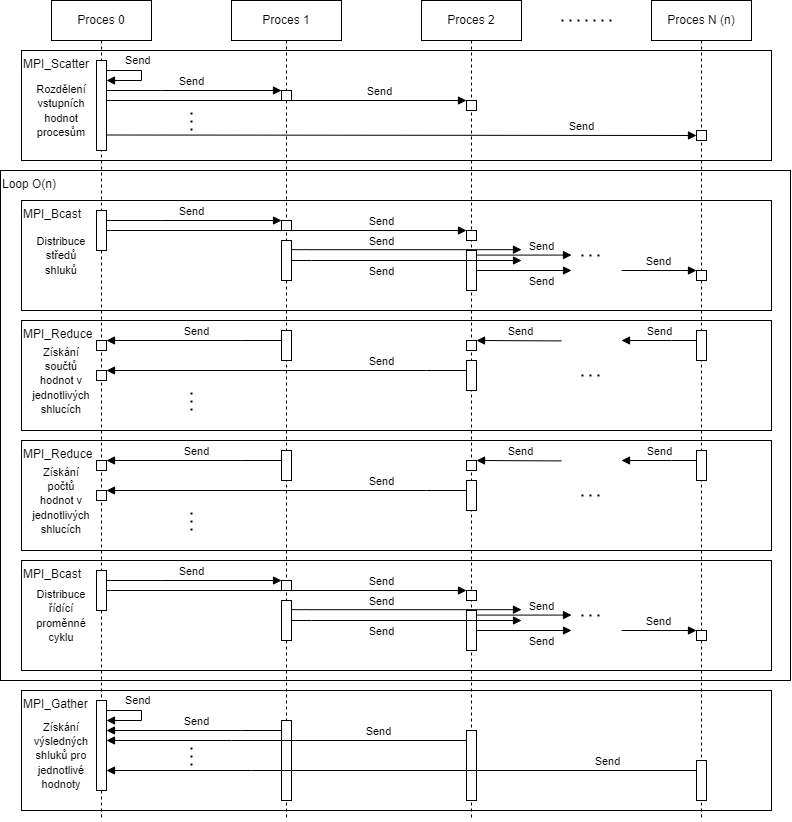
\includegraphics[scale=0.52]{komunikacni-protokol.png}
	\caption{Sekvenční diagram zobrazující komunikační protokol znázorňující komunikaci mezi jednotlivými běžícími procesy implementovaného algoritmu}\label{pic:4-means:seq-diagram}
\end{figure}



\section{Závěr}



V rámci tohoto projektu bylo v \textit{C++} s využitím \textit{Open MPI} úspěšně implementováno paralelní řešení algoritmu 4-means nad skalárními vstupními hodnotami. Pro tuto implementaci byla dále zanalyzována časová složitost, prostorová složitost a celková cena. Bylo zjištěno, že časová složitost tohoto řešení je linearitmická a prostorová složitost je lineární. Cena tohoto paralelního řešení pak není optimální. Zrychlení oproti sekvenčnímu řešení je rovno $\frac{\bigO{n}}{\bigO{\log n}}$, přičemž efektivnost této paralelní implementace odpovídá $\frac{1}{\bigO{\log n}} < 1$.



\end{document}
